\newpage
\section{Generalized Functors}

\subsection{Why we need functors?}


  A generalized functor

\begin{itemize}
\item \textbf{Encapsulates} any processing invocation because it accepts
  pointers to simple functions, pointers to member functions,
  functors, and even other generalized functors—together with some or
  all of their respective arguments.
\item Is \textbf{typesafe} because it never matches the wrong argument
  types to the wrong functions.
\item Is an object with \textbf{value semantics} because it fully
  supports copying, assignment, and pass by value. A generalized
  functor can be copied freely and does not expose virtual member
  functions.
\end{itemize}


A typical sequence of actions is as follows:

\begin{figure}[H]
  \centering
  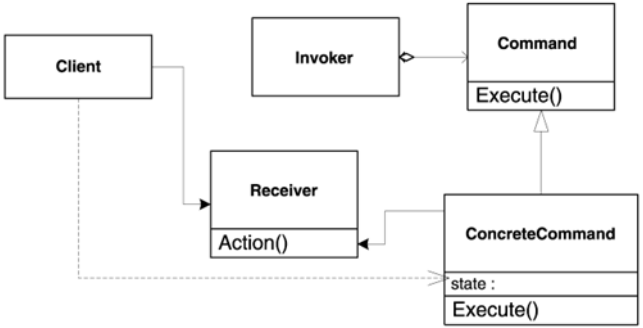
\includegraphics[width = 0.8\textwidth]{5.Functor/Functor1.png}
\end{figure}

\begin{enumerate}
\item The application (client) creates a \texttt{ConcreteCommand}
  object, passing it enough information to carry on a task. 
\item The application passes the \texttt{Command} interface of the
  \texttt{ConcreteCommand} object to the invoker. The invoker stores
  this interface.
\item  the invoker decides it's time to execute the action and fires
  \texttt{Command}'s Execute virtual member function. The virtual call
  mechanism dispatches the call to the \texttt{Concrete-Command }
  object, which takes care of the details. \texttt{ConcreteCommand}
  reaches the \texttt{Receiver} object (the one that is to do the job)
  and uses that object to perform the actual processing, such as
  calling its \texttt{Action } member function. Alternatively, the
  \texttt{ConcreteCommand} object might carry the processing all by
  itself. In this case, the receiver in Figure disappears.
\end{enumerate}

There are two important aspects of the Command pattern:
\begin{itemize}
\item \textbf{Interface separation}. The invoker is isolated from the
  receiver. 
\item \textbf{Time separation}. Command stores a ready-to-go
  processing request that's to be started later.
\end{itemize}

From an implementation standpoint, two kinds of concrete \texttt{Command}
classes can be identified:
\begin{enumerate}
\item All they do is call a member function for a \texttt{Receiver}
  object. We call them \textbf{forwarding commands}.
\item Others do tasks that are more complex. They might call member
functions of other objects, but they also embed logic that's beyond
simple forwarding. Let's call them active commands\textbf{}. 
\end{enumerate}
Because forwarding commands act much
like pointers to functions and their C++ colleagues, functors, we call
them \textbf{generalized functors}. 

\subsection{C++ Callable Entities}

A forwarding command is a callback on steroids, a generalized
callback. A callback is a pointer to a function that can be passed
around and called at any time.

In addition to simple callbacks, C++ defines many more entities that
support the function-call operator.  Let's enumerate all the things
that support \texttt{operator()} in C++:
\begin{itemize}
\item C-like functions
\item C-like pointers to functions
\item References to functions (which essentially act like const
  pointers to functions)
\item Functors, that is, objects that define an \texttt{operator()}
\item The result of applying \texttt{operator.*} or
  \texttt{operator->*} having a pointer to a member function
\end{itemize}
The objects that support \texttt{operator()} are known as
\textbf{callable entities}.

\subsection{\texttt{Functor} Class Template Skeleton}

in C++ a bald pointer to a polymorphic type does not strictly have first-class
semantics because of the ownership issue. To lift the burden of
lifetime management from \texttt{Functor}'s clients, it's best to provide
\texttt{Functor} with value semantics (well-defined copying and assignment).
\texttt{Functor} does have a polymorphic implementation, but that's hidden
inside it. We name the implementation base class \texttt{FunctorImpl}.

\begin{verbatim}
template <typename R, class TList>
class Functor{
public:
  Functor();
  Functor(const Functor&);
  Functor& operator=(const Functor&);
  explicit Functor(std::auto_ptr<Impl> spImpl);
private:
  // Handy type definition for the body type
  typedef FunctorImpl<R, TList> Impl;
  std::auto_ptr<Impl> spImpl_;
};
\end{verbatim}
The purpose of \texttt{Clone} is the creation of a polymorphic copy of
the \texttt{FunctorImpl} object.

\texttt{FunctorImpl} defines a polymorphic interface that abstracts a
function call.

\begin{verbatim}
template <typename R>
class FunctorImpl<R, NullType>{
public:
  virtual R operator()() = 0;
  virtual FunctorImpl* Clone() const = 0;
  virtual ~FunctorImpl() {}
};
template <typename R, typename P1>
class FunctorImpl<R, TYPELIST_1(P1)>{
public:
  virtual R operator()(P1) = 0;
  virtual FunctorImpl* Clone() const = 0;
  virtual ~FunctorImpl() {}
};
template <typename R, typename P1, typename P2>
class FunctorImpl<R, TYPELIST_2(P1, P2)>{
public:
  virtual R operator()(P1, P2) = 0;
  virtual FunctorImpl* Clone() const = 0;
  virtual ~FunctorImpl() {}
};
\end{verbatim}

Constructing from \texttt{auto\_ptr} is a clear statement to the
outside world that \texttt{Functor} takes ownership of 
the \texttt{FunctorImpl} object. Users of \texttt{Functor} will
actually have to type \texttt{auto\_ptr} whenever they invoke 
this constructor; we assume that if they type \texttt{auto\_ptr}, they
know what \texttt{auto\_ptr} is about.

\subsection{Implementing the Forwarding \texttt{Functor::operator()}}

\begin{verbatim}
template <typename R, class TList>
class Functor{
... as above ...
public:
  R operator()(){  return (*spImpl_)(); }
  R operator()(Parm1 p1){  return (*spImpl_)(p1); }
  R operator()(Parm1 p1, Parm2 p2){  return (*spImpl_)(p1, p2); }
};
\end{verbatim}

The  trick relies on the fact that \textbf{C++ does not instantiate member
  functions for templates until they are actually used}. If you try to call an overload
of \texttt{operator()} that doesn't make sense, the compiler tries to generate
the body of \texttt{operator()} and discovers the mismatch.

\subsection{Handling Functors}

\begin{verbatim}
template <class ParentFunctor, typename Fun>
class FunctorHandler: public FunctorImpl<
                       typename ParentFunctor::ResultType, 
                       typename ParentFunctor::ParmList>{
public:
  typedef typename ParentFunctor::ResultType ResultType;
  FunctorHandler(const Fun& fun) : fun_(fun) {}
  FunctorHandler* Clone() const{ 
    return new FunctorHandler(*this); 
  }
  ResultType operator()(){
    return fun_();
  }
  ResultType operator()(typename ParentFunctor::Parm1 p1){
    return fun_(p1);
  }
  ResultType operator()(typename ParentFunctor::Parm1 p1,typename ParentFunctor::Parm2 p2){
    return fun_(p1, p2);
  }
private:
  Fun fun_;
};
\end{verbatim}

The functor is stored by value, not by pointer. This is because, in general,
functors are meant to be this way—nonpolymorphic types with regular
copy semantics.

Given \texttt{FunctorHandler}'s declaration, it's easy to write the templated
constructor of \texttt{Functor} declared earlier in this section.

\begin{verbatim}
template <typename R, class TList>
template <typename Fun>
Functor<R, TList>::Functor(const Fun& fun) : spImpl_(new FunctorHandler<Functor, Fun>(fun)){}
\end{verbatim}

\textbf{\texttt{FuncotHandler} not only handles functor, function but
  also pointer and reference to functions.}

However, if the function is \textbf{overloaded}, the type of the function is no
longer defined.
\begin{verbatim}
void TestFunction(int i, double d){ cout << "TestFunction << endl; }
void TestFunction(int);
\end{verbatim}

There are two methods:
\begin{verbatim}
int main()
{
typedef void (*TpFun)(int, double);
// Method 1: use an initialization
TpFun pF = TestFunction;
Functor<void, TYPELIST_2(int, double)> cmd1(pF);
cmd1(4, 4.5);

// Method 2: use a cast
Functor<void, int, double> cmd2(static_cast<TpFun>(TestFunction));
cmd2(4, 4.5);
}
\end{verbatim}

\subsection{Argument and Return Type Conversions}

In an ideal world, we would like conversions to work for \texttt{Functor} just
as they work for regular function calls. 
\begin{verbatim}
const char* TestFunction(double, double){
  static const char buffer[] = "Hello, world!";
// It's safe to return a pointer to a static buffer
  return buffer;
}
int main(){
  Functor<string, TYPELIST_2(int, int)> cmd(TestFunction);
  // Should print "world!"
  cout << cmd(10, 10).substr(7);
}
\end{verbatim}

The function
\begin{verbatim}
string Functor<...>::operator()(int i, int j)
\end{verbatim}
forwards to the virtual function
\begin{verbatim}
string FunctorHandler<...>::operator()(int i, int j)
\end{verbatim}
whose implementation ultimately calls
\begin{verbatim}
return fun_(i, j);
\end{verbatim}
where \texttt{fun\_} has type \texttt{const char* (*)(double, double)}
and evaluates to \texttt{TestFunction}. When the compiler encounters
the call to \texttt{fun\_}, it compiles it normally. The compiler then
generates code to convert \texttt{i} and \texttt{j} to
\texttt{double}, and the result to \texttt{std::string}.

\subsection{Handling Pointers to Member Functions}

\begin{verbatim}
class Parrot{
public:
void Eat(){ cout << "Tsk, knick, tsk...\n"; }
void Speak(){ cout << "Oh Captain, my Captain!\n"; }
};
int main(){
  typedef void (Parrot::* TpMemFun)();
  TpMemFun pActivity = &Parrot::eat;
  
  Parrot geronimo;
  Parrot* pGeronimo = &geronimo;
  (geronimo.*pActivity)();
  (pGeronimo->*pActivity)();
  pActivity = &Parrot::Speak;
  (geronimo.*pActivity)();
}
\end{verbatim}

There is no C++ type for the result of \texttt{geronimo.*p-Activity}
and \texttt{pGeronimo->*pActivity}. Both are binary operations all
right, and they return something to which you can apply the 
function-call operator immediately, but that "something" does not have
a type. You cannot store the result of \texttt{operator.*} or
\texttt{operator->*} in any way.

Here's the implementation of \texttt{MemFunHandler}.
\begin{verbatim}
template <class ParentFunctor, typename PointerToObj, typename PointerToMemFn>
class MemFunHandler : public FunctorImpl<
                       typename ParentFunctor::ResultType,
                       typename ParentFunctor::ParmList>{
public:
  typedef typename ParentFunctor::ResultType ResultType;

  MemFunHandler(const PointerToObj& pObj, PointerToMemFn pMemFn) : pObj_(pObj), pMemFn_(pMemFn) {}
  MemFunHandler* Clone() const{ 
    return new MemFunHandler(*this); 
  }

  ResultType operator()(){
    return ((*pObj_).*pMemFn_)();
  }
  ResultType operator()(typename ParentFunctor::Parm1 p1){
    return ((*pObj_).*pMemFn_)(p1);
  }
ResultType operator()(typename ParentFunctor::Parm1 p1, typename ParentFunctor::Parm2 p2){
    return ((*pObj_).*pMemFn_)(p1, p2);
  }
private:
  PointerToObj pObj_;
  PointerToMemFn pMemFn_;
};
\end{verbatim}

Why is \texttt{MemFunHandler} parameterized with the type of the
pointer (\texttt{PointerToObj}) and not with the  type of the object
itself? i.e.
\begin{verbatim}
template <class ParentFunctor, typename Obj,
typename PointerToMemFn>
class MemFunHandler : public FunctorImpl<
                       typename ParentFunctor::ResultType,
                       typename ParentFunctor::ParmList>{
private:
  Obj* pObj_;
  PointerToMemFn pMemFn_;
public:
MemFunHandler(Obj* pObj, PointerToMemFn pMemFn) : pObj_(pObj), pMemFn_(pMemFn) {}
};
\end{verbatim}

The first implementation can store any type that acts as a pointer to an
object \textbf{but} the second is hardwired to store and use only
simple pointers, if you want to use smart pointers, there will be
wrong.

Moreover, the second version does not work for pointers to
\texttt{const}. Such is the negative effect of hardwiring type.

\begin{verbatim}
int main(){
  Parrot geronimo;
  Functor<> cmd1(&geronimo, &Parrot::Eat), cmd2(&geronimo, &Parrot::Speak);
  cmd1();
  cmd2();
}
\end{verbatim}
%%% Local Variables:
%%% mode: latex
%%% TeX-master: "../DesignPattern"
%%% End:
